\documentclass[10pt]{scrartcl}
    % General document formatting
    \usepackage[margin=0.7in]{geometry}
    \usepackage[parfill]{parskip}
    \usepackage[utf8]{inputenc}
    \usepackage[ngerman]{babel}
    \usepackage{graphicx}
    \usepackage{subcaption}
    \usepackage{times}
    \usepackage{hyperref}
    
    % Related to math
    \usepackage{amsmath,amssymb,amsfonts,amsthm}

\begin{document}
\title{Deep Learning Lab Course}
\subtitle{Imitation Learning and Reinforcement Learning}
\author{Jonas Kölblin, Matr.-Nr. 5763431}
\date{May 2, 2024}
\maketitle

% \section*{Introduction}


\section{Imitation Learning}
\subsection{Getting familiar with the environment}
After installing the last stubborn dependency box2d, I was able to run the provided code. The stearing mechanics were a bit difficult to get used to but after a few runs I felt confident enough to start collecting training data. 

\subsection{Collecting training data}
While collecting data I implemented the first changes to the provided code. I made the data collecting more convenient by printing, how many data points have been collected so far, and by making the game pause while the data is being saved, so one is not immediately thrown back into the game after the screen freezes for a long time. Unfortunately, I collected the data in multiple runs and realized too late that the data was overwritten each time. So I also changed the saving function to append the data to the file instead of overwriting it. After collecting about 30.000 samples, I moved on to the next step. \\
Later I realized that the action \dq break\dq{} was not saved or recognized by the action to id function. This was also the case for other students. Unfortunately, I did not have the time to fix this issue, so I had to adapt the number of classes to 4.

\subsection{Training a Behavioral Cloning Agent}
The first training already looked promising in terms of metrics (see figure \ref{fig:Il1}). However when looking at the test results it became obvious that the network was just overfitting on the action \dq straight\dq{} which made up a large percentage of the dataset. The testing result had a mean score of 67.3 and a standard deviation of 54.5. \\
Hyperparameters: cross-entropy loss, Adam optimizer, learning rate 0.001, batch size 64, 1000 batch steps, 60000 samples.

\subsection{Improving the Behavioral Cloning Agent}
To improve the agent I had to make sure that the validation set did not only consist of the action \dq straight\dq , so I replaced the existing splitting method with the "train\_test\_split" method from sklearn. This method supports stratification which makes sure that the distribution of the actions is the same in the training and validation set. \\
Furthermore, I implemented a class-weighted batch sampling method instead of the suggested uniform sampling, so I had some more control over the distribution of the actions in the training set. To find a good configuration for the class weights I implemented a random search algorithm and ran 100 evaluations with a shortened training length of 300 batch steps. The best configuration I found was 4, 2, 2, 3 (straight, left, right, accelerate). I also experimented with other learning rates and sgd-optimizer but the Adam optimizer with a learning rate of 0.001 still performed best. \\
Next I collected much more data, over 200.000 samples, hoping that this would lead to better generalization. I underestimated the memory requirements of this much data and so I could never train the network on the full dataset. Implementing some kind of lazy loading would have been a good idea but for that huge changes to the training pipeline would have been necessary. \\
Then I started training the network with history length 1. The training results were worse than expected (see figure \ref{fig:Il_hl1}). The agent reached a mean score of 365.3 with a standard deviation of 199.6. This was devestating considering that the training took about 36h.
Hyperparameters: cross-entropy loss, Adam optimizer, learning rate 0.001, batch size 64, 500000 batch steps, 135000 samples \\
After this I optimzed the code and moved every calculation to the GPU. With these optimizations my next training with history length 3 was much faster. The results were also better (see figure \ref{fig:Il_hl3}). The test performance was still not good with a mean of 408.3 and a standard deviation of 175.3. The agent was able to follow the track nicely but it was driving very slow sometimes and also got lost a few times. Hyperparameters: cross-entropy loss, Adam optimizer, learning rate 0.0001, batch size 64, 200000 batch steps, 95000 samples.
Finally I tried to train the network with a history length of 5 but I had to reduce number of samples to 75000 because of memory issues. The results were not better than with history length 3 (see figure \ref{fig:Il_hl5}). However during testing the additional history length made a difference. The agent reached a mean score of 585.6 with a standard deviation of 106.4. Hyperparameters: cross-entropy loss, Adam optimizer, learning rate 0.0001, batch size 64, 200000 batch steps, 75000 samples.
\subsection*{Conclusion}
Despite having collected tons of data I was only able to archieve mediocre testing performance due to memory restrictions and the lack of time to play around with the hyperparameters more or add other kinds of regularization. I think that the ability to break would also improve the performance of the agent. Also the action \dq accelerate\dq{} should be emphasized more in the training data so the agent is not only able to follow the track but also to drive faster.

\section{Reinforcement Learning: Deep Q-Networks}
\subsection{CartPole}
Having learned from the Imitation Learning history length 1 training I directly implemented everything (including the replay buffer) on the GPU. The CartPole training is visualized in figure \ref{fig:Rl_cp}. Although the reward per episode does not look that smooth the agent was able to archive a mean score of 202 with a standard deviation of 0.0 during testing. Hyperparameters were chosen as provided in the code with replay buffer size of 1e6 and 3000 training episodes.

\subsection{CarRacing}
The first training went terrible (see figure \ref{fig:Rl_hl1}). The agent got even worse over time. While testing it only drove in circles. The mean score was -76.6 with a standard deviation of 2.2. Hyperparameters were chosen as provided in the code with replay buffer size of 1e5 and the training was stopped after around 700 episodes. \\
After my experiences with the Imitation Learning agent I decided to directly increase the history length to 3 instead of trying to archieve a good score with history length 1. I also implemented the suggestions frame skipping, increasing episode length and weighted probabilities for exploration. The training looked very promising (see figure \ref{fig:Rl_hl3}). Unfortunately the training crashed after close to 700 episodes because the memory of my GPU was full. The agent was able to archive a mean score of 360.2 with a standard deviation of 284.7. The problem was mainly that the agent was going too fast most of the time, overshot the curves and the got lost. Hyperparameters changed: epsilon 0.2 with 0.99 decay, replay buffer size 1e5, skip frames 2, max episode length 200 + i for shorter episodes in the beginning, exploration weights 5, 2, 2, 4, 1 (straight, left, right, accelerate, break). \\
After that I tried to run a training with history length 5 and reduced the replay buffer size to 1e4 to make it work with my GPU memory. The training was stopped early after 160 episodes because it was obvious that the agent was not learning anything (see figure \ref{fig:Rl_hl5}). I also tried a run with a history length of 2 but the results were not better than with history length 3. Hyperparameters changed: epsilon 0.2 with 0.99 decay, replay buffer size 1e4, skip frames 2, max episode length 200 + i for shorter episodes in the beginning, exploration weights 5, 2, 2, 4, 1 (straight, left, right, accelerate, break).

\subsection{Conclusion}
Sadly my most promising training crashed because of memory issues and I was not able to find a good solution for this problem in the given time. I think the replay buffer should maybe be implemented on CPU to save GPU memory but I was not able to implement this without excessive switching of tensors between the processing units which would result in long training times. I am convinced that the hyperparameters were good because the reward per episode showed decent growth and no sign of convergence.

\section{Outlook}
From the beginning of this task on I planned to enter the competition with my agents, that was the reason why I collected so much data and tried to optimize the agents as much as possible. My plan for my final competing agent was to warm start a DQN training with my best Imitation Learning network. I think this would have been a good idea because the Imitation Learning agent was able to follow the track nicely and the DQN agent was able to drive fast. Unfortunately this was difficult due to several reasons. First of all the Imitation Learning agent was not able to break, so the number of outputs differed which made loading the weights into the DQN training difficult. Also the memory issues of my implementation made it impossible to train the DQN agent sufficiently. Finally I didn't have enough time at the end to overcome these issues. So I gave up on the competition and focused on finishing the documentation. But I think that the warm starting would have been a good idea and I am looking forward to see if someone else had the same idea and how well it worked out.

\newpage
\section*{Appendix}
Github repository: \url{https://github.com/Bicyclettamanagement/dl-lab-ilrl}\\
% images
\begin{figure}[h]
\begin{subfigure}{0.5\textwidth}
  \centering
  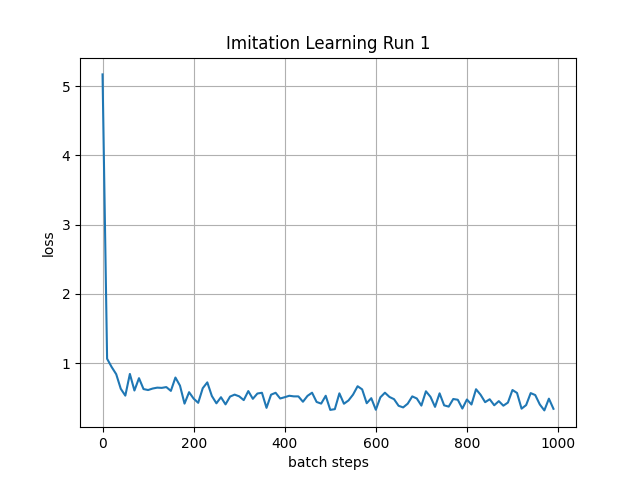
\includegraphics[width=\linewidth]{images/Il1_loss.png}
  \caption{Loss}
  \label{fig:Il1_loss}
\end{subfigure} 
\begin{subfigure}{0.5\textwidth}
  \centering
  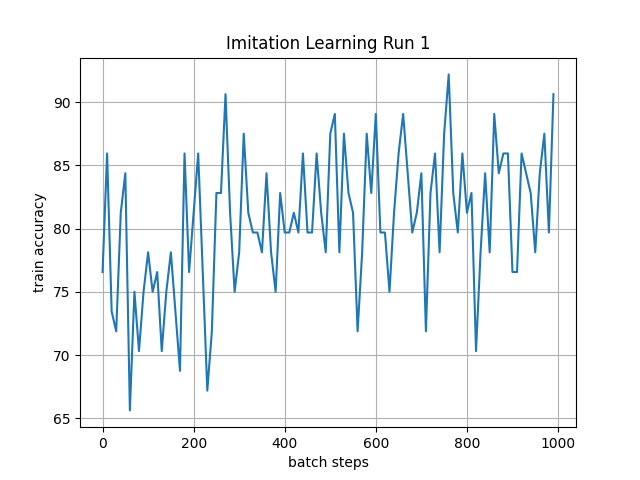
\includegraphics[width=\linewidth]{images/Il1_train.png}
  \caption{Training Accuracy}
  \label{fig:Il1_train}
\end{subfigure} \\
\begin{subfigure}{0.5\textwidth}
  \centering
  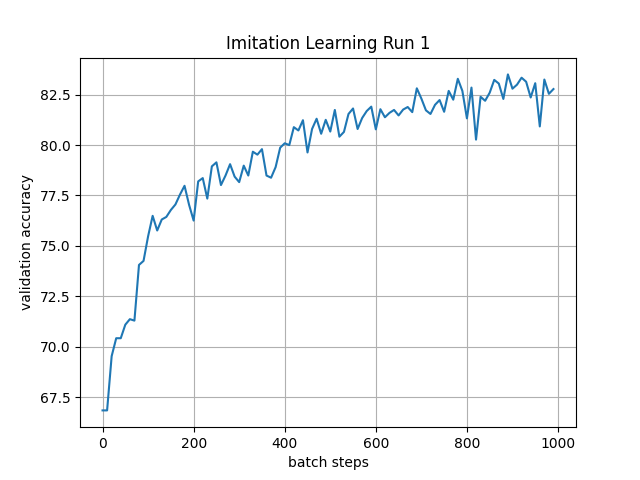
\includegraphics[width=\linewidth]{images/Il1_valid.png}
  \caption{Validation Accuracy}
  \label{fig:Il1_valid}
\end{subfigure}
\caption{Training results of the first Imitation Learning agent}
\label{fig:Il1}
\end{figure}

\begin{figure}[h]
    \begin{subfigure}{0.5\textwidth}
      \centering
      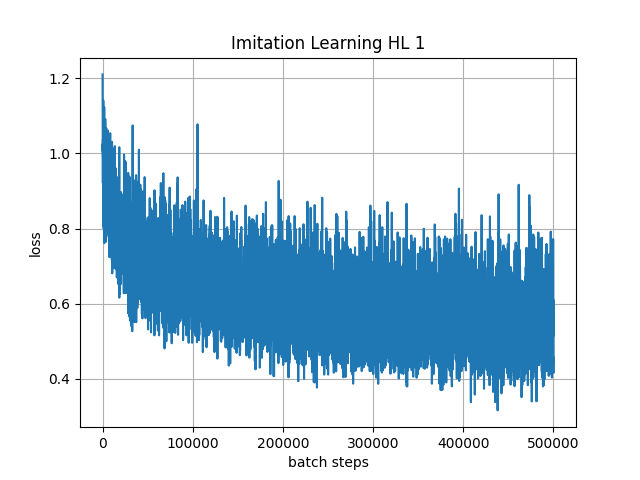
\includegraphics[width=\linewidth]{images/Il_hl1_loss.png}
      \caption{Loss}
      \label{fig:Il_hl1_loss}
    \end{subfigure} 
    \begin{subfigure}{0.5\textwidth}
      \centering
      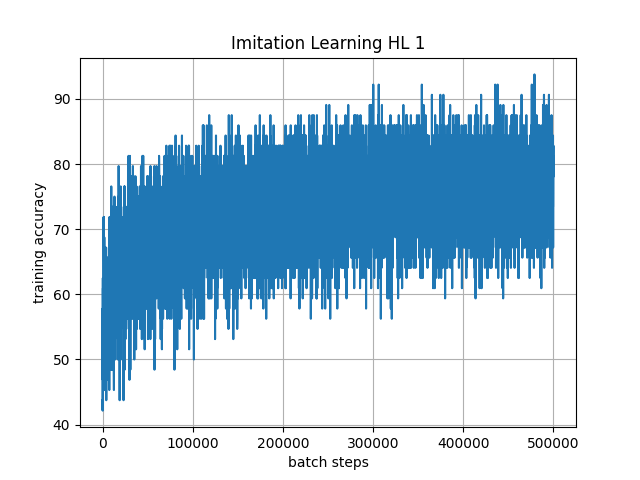
\includegraphics[width=\linewidth]{images/Il_hl1_train.png}
      \caption{Training Accuracy}
      \label{fig:Il_hl1_train}
    \end{subfigure} \\
    \begin{subfigure}{0.5\textwidth}
      \centering
      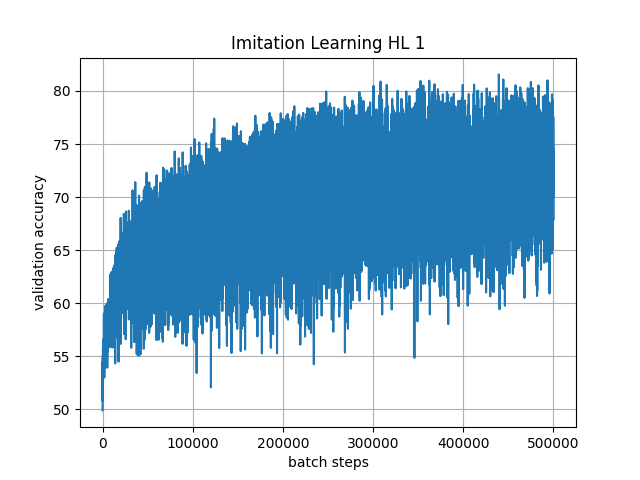
\includegraphics[width=\linewidth]{images/Il_hl1_valid.png}
      \caption{Validation Accuracy}
      \label{fig:Il_hl1_valid}
    \end{subfigure}
    \caption{Training results with history length 1}
    \label{fig:Il_hl1}
\end{figure}
\begin{figure}[h]
    \begin{subfigure}{0.5\textwidth}
      \centering
      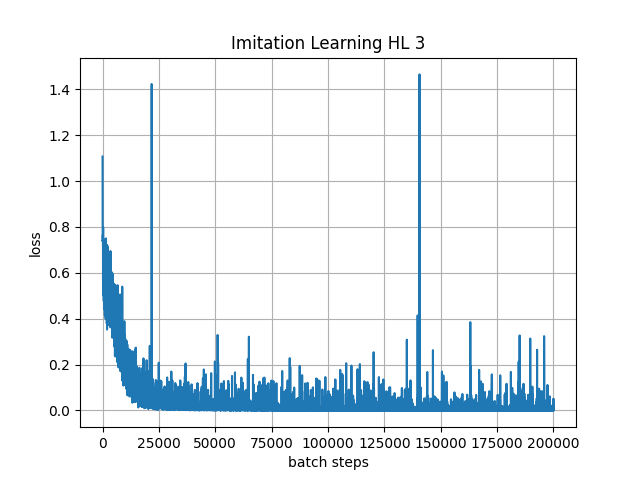
\includegraphics[width=\linewidth]{images/Il_hl3_loss.png}
      \caption{Loss}
      \label{fig:Il_hl3_loss}
    \end{subfigure} 
    \begin{subfigure}{0.5\textwidth}
      \centering
      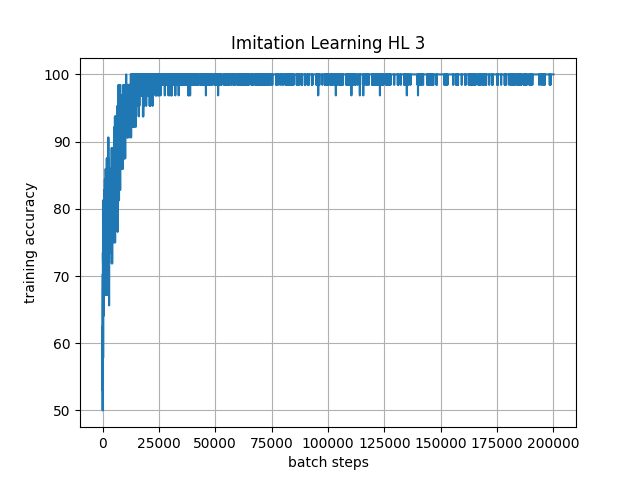
\includegraphics[width=\linewidth]{images/Il_hl3_train.png}
      \caption{Training Accuracy}
      \label{fig:Il_hl3_train}
    \end{subfigure} \\
    \begin{subfigure}{0.5\textwidth}
      \centering
      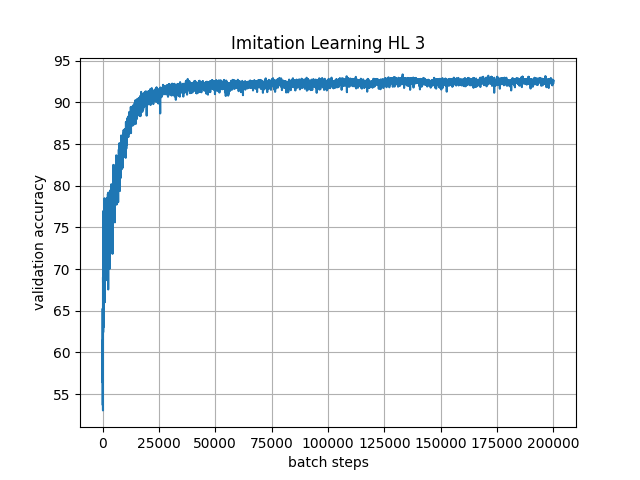
\includegraphics[width=\linewidth]{images/Il_hl3_valid.png}
      \caption{Validation Accuracy}
      \label{fig:Il_hl3_valid}
    \end{subfigure}
    \caption{Training results with history length 3}
    \label{fig:Il_hl3}
\end{figure}
\begin{figure}[h]
    \begin{subfigure}{0.5\textwidth}
      \centering
      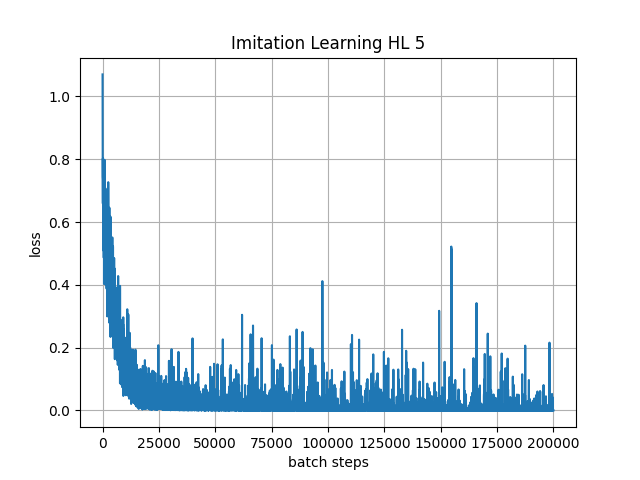
\includegraphics[width=\linewidth]{images/Il_hl5_loss.png}
      \caption{Loss}
      \label{fig:Il_hl5_loss}
    \end{subfigure} 
    \begin{subfigure}{0.5\textwidth}
      \centering
      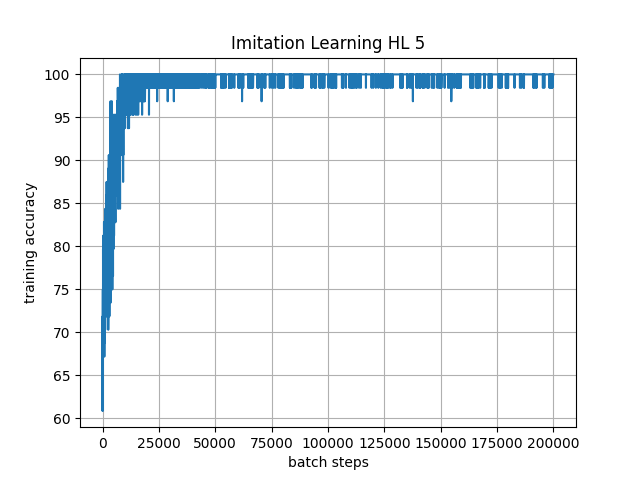
\includegraphics[width=\linewidth]{images/Il_hl5_train.png}
      \caption{Training Accuracy}
      \label{fig:Il_hl5_train}
    \end{subfigure} \\
    \begin{subfigure}{0.5\textwidth}
      \centering
      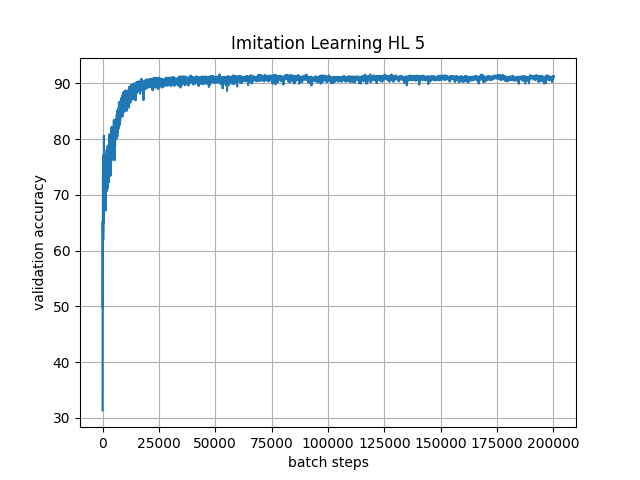
\includegraphics[width=\linewidth]{images/Il_hl5_valid.png}
      \caption{Validation Accuracy}
      \label{fig:Il_hl5_valid}
    \end{subfigure}
    \caption{Training results with history length 5}
    \label{fig:Il_hl5}
\end{figure}
\begin{figure}[h]
    \centering
    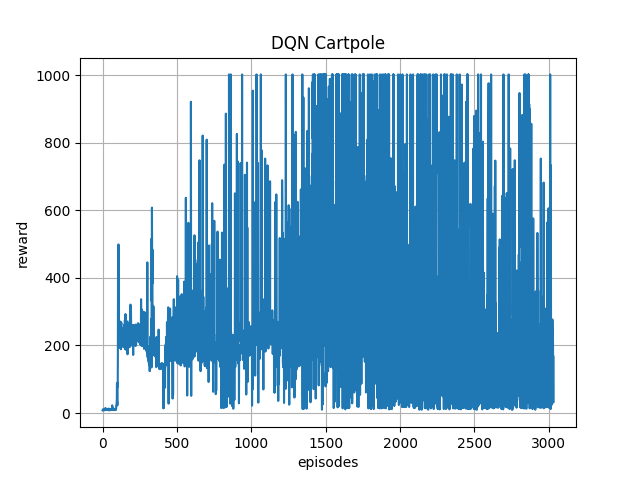
\includegraphics[width=0.5\linewidth]{images/RL_cp.png}
    \caption{Training results of the CartPole agent}
    \label{fig:Rl_cp}
\end{figure}
\begin{figure}[h]
    \begin{subfigure}{0.5\textwidth}
      \centering
      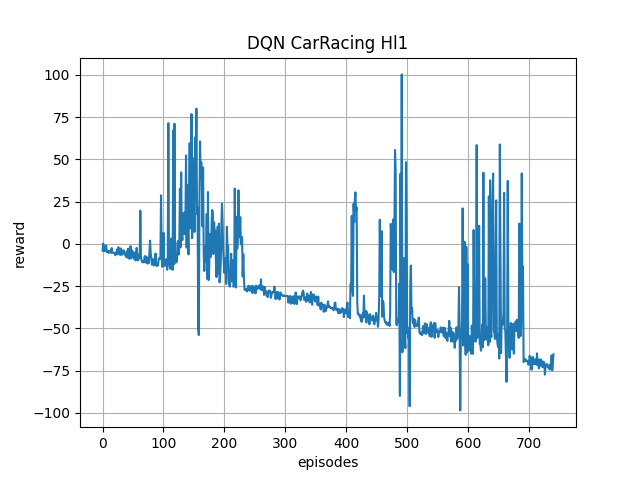
\includegraphics[width=\linewidth]{images/RL_hl1.png}
      \caption{Training}
      \label{fig:RL_hl1_train}
    \end{subfigure} 
    \begin{subfigure}{0.5\textwidth}
      \centering
      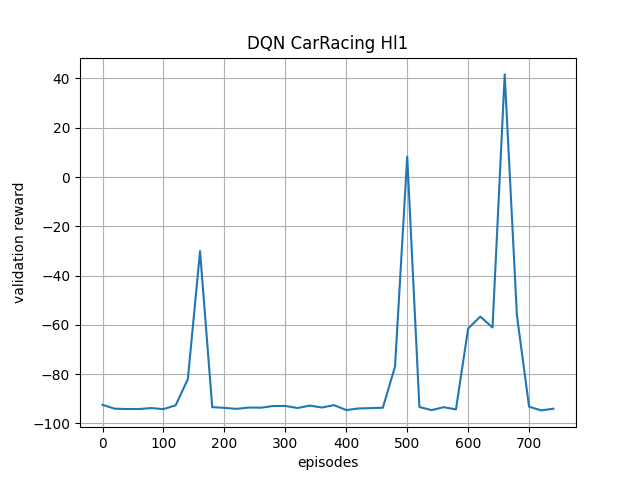
\includegraphics[width=\linewidth]{images/RL_hl1_val.png}
      \caption{Validation}
      \label{fig:RL_hl1_val}
    \end{subfigure}
    \caption{Training results of the CarRacing agent with history length 1}
    \label{fig:Rl_hl1}
\end{figure}
\begin{figure}[h]
    \begin{subfigure}{0.5\textwidth}
      \centering
      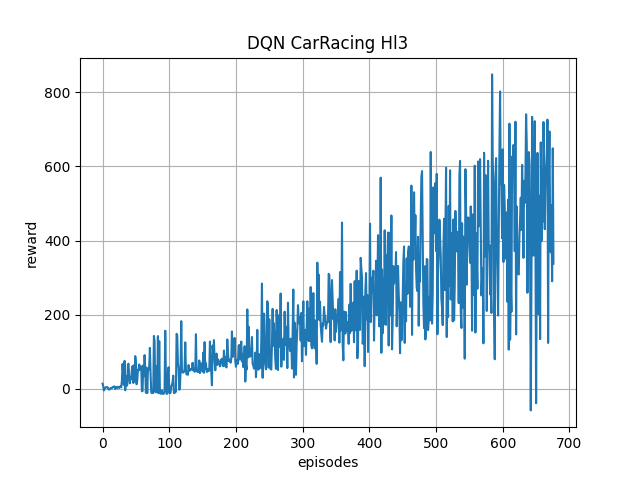
\includegraphics[width=\linewidth]{images/RL_hl3.png}
      \caption{Training}
      \label{fig:RL_hl3_train}
    \end{subfigure} 
    \begin{subfigure}{0.5\textwidth}
      \centering
      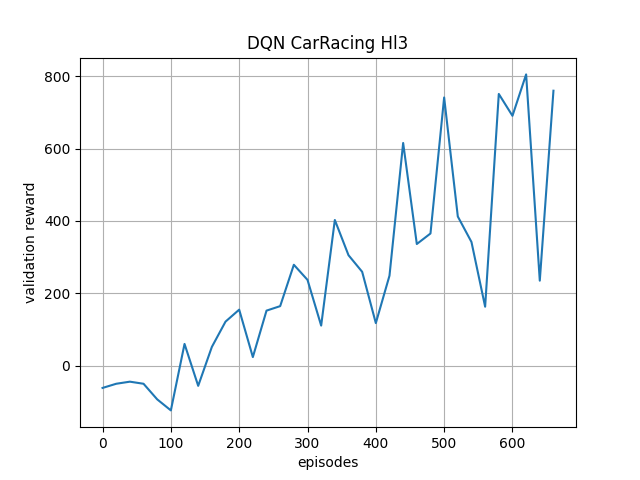
\includegraphics[width=\linewidth]{images/RL_hl3_val.png}
      \caption{Validation}
      \label{fig:RL_hl3_val}
    \end{subfigure}
    \caption{Training results of the CarRacing agent with history length 3}
    \label{fig:Rl_hl3}
\end{figure}
\begin{figure}[h]
    \begin{subfigure}{0.5\textwidth}
      \centering
      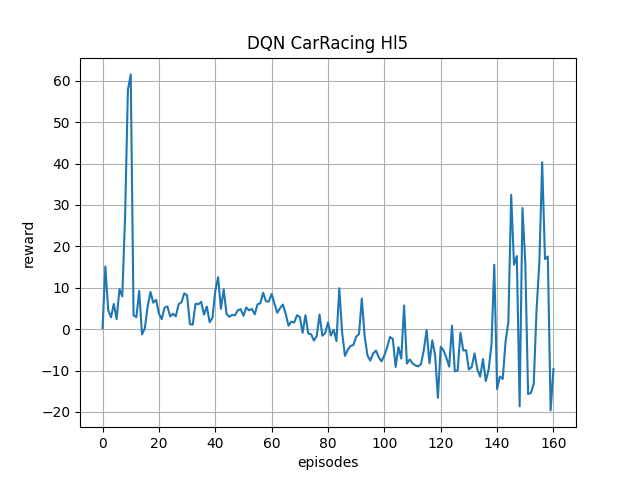
\includegraphics[width=\linewidth]{images/RL_hl5.png}
      \caption{Training}
      \label{fig:RL_hl5_train}
    \end{subfigure} 
    \begin{subfigure}{0.5\textwidth}
      \centering
      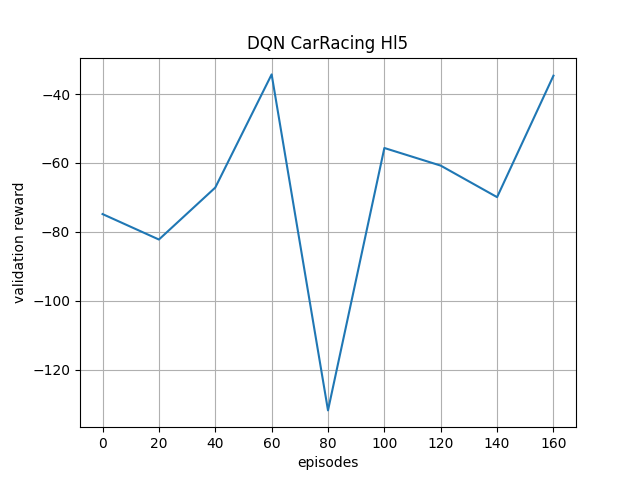
\includegraphics[width=\linewidth]{images/RL_hl5_val.png}
      \caption{Validation}
      \label{fig:RL_hl5_val}
    \end{subfigure}
    \caption{Training results of the CarRacing agent with history length 5}
    \label{fig:Rl_hl3}
\end{figure}

\end{document}